\documentclass[xcolor={x11names}]{beamer}

% \usetheme{Frankfurt}

% \setbeameroption{show notes}
% \setbeamertemplate{note page}[plain]

\usetheme{Boadilla}
\usecolortheme{whale}

% \usetheme{Madrid}
% \useoutertheme{miniframes} % Alternatively: miniframes, infolines, split
% \useinnertheme{circles}

\usepackage[T1]{fontenc}
\usepackage[utf8]{inputenc}
\usepackage[french,english]{babel}

\usepackage{blindtext}
\usepackage{appendixnumberbeamer}
\usepackage{graphicx}
\usepackage{xcolor}
\usepackage{listings}

%% Listing colors
\definecolor{codegreen}{rgb}{0,0.6,0}
\definecolor{codegray}{rgb}{0.5,0.5,0.5}
\definecolor{codepurple}{rgb}{0.58,0,0.82}
\definecolor{codeblue}{rgb}{0.10,0,0.82}
\definecolor{codebackcolour}{rgb}{0.95,0.95,0.92}

\usepackage{tikz}
\usetikzlibrary{positioning}
\usetikzlibrary{matrix}
\usetikzlibrary{shapes.multipart}
\tikzset{
    invisible/.style={opacity=0,%
    prefix after command={\pgfextra{\tikzset{every label/.style={opacity=0}}}}},
    visible on/.style={alt={#1{}{invisible}}},
    alt/.code args={<#1>#2#3}{%
        \alt<#1>{\pgfkeysalso{#2}}{\pgfkeysalso{#3}}
    },
    onslide/.code args={<#1>#2}{%
        \only<#1>{\pgfkeysalso{#2}}
    },
    temporal/.code args={<#1>#2#3#4}{%
        \temporal<#1>{\pgfkeysalso{#2}}{\pgfkeysalso{#3}}{\pgfkeysalso{#4}}
    },
    von/.code args={<#1>}{%
        \alt<#1>{\pgfkeysalso{opacity=1}}{\pgfkeysalso{opacity=.2}}
    },
}

\def\cov<#1>{\alt<#1>{\color{black!20}}{\color{black}}}
\def\uncov<#1>{\alt<#1>{\color{black}}{\color{black!20}}}

\title[Soutenance de PFE]{Experiments on automation of formal verification of devices at the binary level}
\subtitle{}
\author{Thomas Lacroix}
\titlegraphic{
\includegraphics[width=4cm]{logos/insa-logo-coul.png}}
\institute[]{INSA Lyon \\ Soutenance de PFE (Option R\&D)}
\date[19/06/2019]{Wednesday, June 19, 2019}

\newcommand{\htriple}[3]{\ensuremath{\{#1\}~#2~\{#3\}}}
\newcommand{\WP}{\ensuremath{\mathit{WP}}}
\newcommand{\eqdef}{\ensuremath{\stackrel{def}{=}}}

% Add pages before every section and subsections
\AtBeginSection[]{\frame{\sectionpage}}
\AtBeginSubsection[]
{%
    \begin{frame}
        \frametitle{Table of Contents}
        \tableofcontents[hideothersubsections, currentsection, currentsubsection]
    \end{frame}
}

% Add page number in upper-right corner
% \makeatletter
% \defbeamertemplate*{headline}{my smoothbars theme}
% {%
%     \pgfuseshading{beamer@barshade}%
%     \ifbeamer@sb@subsection%
%     \vskip-9.75ex%
%     \else%
%     \vskip-7ex%
%     \fi%
%     \begin{beamercolorbox}[ignorebg,ht=2.25ex,dp=3.75ex]{section in head/foot}
%     \insertnavigation{.9\paperwidth}\hfill%
%     \insertframenumber/\inserttotalframenumber%
%     \hspace{.5em}
%     \end{beamercolorbox}%
%     \ifbeamer@sb@subsection%
%     \begin{beamercolorbox}[ignorebg,ht=2.125ex,dp=1.125ex,%
%         leftskip=.3cm,rightskip=.3cm plus1fil]{subsection in head/foot}
%         \usebeamerfont{subsection in head/foot}\insertsubsectionhead
%     \end{beamercolorbox}%
%     \fi%
% }%
% \makeatother

% To remove the navigation buttons at the bottom
% \beamertemplatenavigationsymbolsempty

% Explain NIC and what we want to prove
%   - obvious reason: connected to Internet and DMA access
%   - buffer descriptor
%       - not circular
%       - only readable memory
%       - not overlapping
%   - show that it's possible to violate the invariant
%       -> overlapping tx and rx BD
%   => need to model the spec
%   => modeled with invariants
%
% Can we reuse work done for software verification to verify hardware?
%
% Start with explanation of PP analysis vs non-PP
%
% Last 5 minutes, show every supporting tools
%   => everything that is needed that is not direct PP stuff

%%%%%%%%%%%%%%%%%%%%%%%%%%%%%%%%%%%%%%%%%%%%%%%%%%%%%%%%%%%%%%%%%%%%%%%%%%%%%%%%
%%%%%%%%%%%%%%%%%%%%%%%%%%%%%%%%%%%%%%%%%%%%%%%%%%%%%%%%%%%%%%%%%%%%%%%%%%%%%%%%
%%%%%%%%%%%%%%%%%%%%%%%%%%%%%%%%%%%%%%%%%%%%%%%%%%%%%%%%%%%%%%%%%%%%%%%%%%%%%%%%

\begin{document}

\begin{frame}
    \maketitle
\end{frame}

%%%%%%%%%%%%%%%%%%%%%%%%%%%%%%%%%%%%%%%%%%%%%%%%%%%%%%%%%%%%%%%%%%%%%%%%%%%%%%%%
%%%%%%%%%%%%%%%%%%%%%%%%%%%%%%%%%%%%%%%%%%%%%%%%%%%%%%%%%%%%%%%%%%%%%%%%%%%%%%%%
%%%%%%%%%%%%%%%%%%%%%%%%%%%%%%%%%%%%%%%%%%%%%%%%%%%%%%%%%%%%%%%%%%%%%%%%%%%%%%%%

\section{Motivation}

%%%%%%%%%%%%%%%%%%%%%%%%%%%%%%%%%%%%%%%%%%%%%%%%%%%%%%%%%%%%%%%%%%%%%%%%%%%%%%%%

\subsection{Security critical systems}

\begin{frame}{Security critical systems}
    \begin{columns}
        \begin{column}{0.5\textwidth}
            Privacy

            \begin{itemize}
                \item Smartphones
                \item Smart TVs
            \end{itemize}
        \end{column}
        \begin{column}{0.5\textwidth}
            Integrity

            \begin{itemize}
                \item Hospital equipment
                \item Traffic control systems
                \item Power plants
            \end{itemize}
        \end{column}
    \end{columns}

    \vfill
    \pause

    \note{Systems are getting more and more complex with time, and}
    \textbf{Problem}: complex systems almost always contain bugs
    \note{bugs => vulnerabilities}
\end{frame}

\begin{frame}{Security critical systems - vulnerable}
    \pause
    \begin{columns}
        \begin{column}{0.5\textwidth}
            \begin{figure}
                \centering
                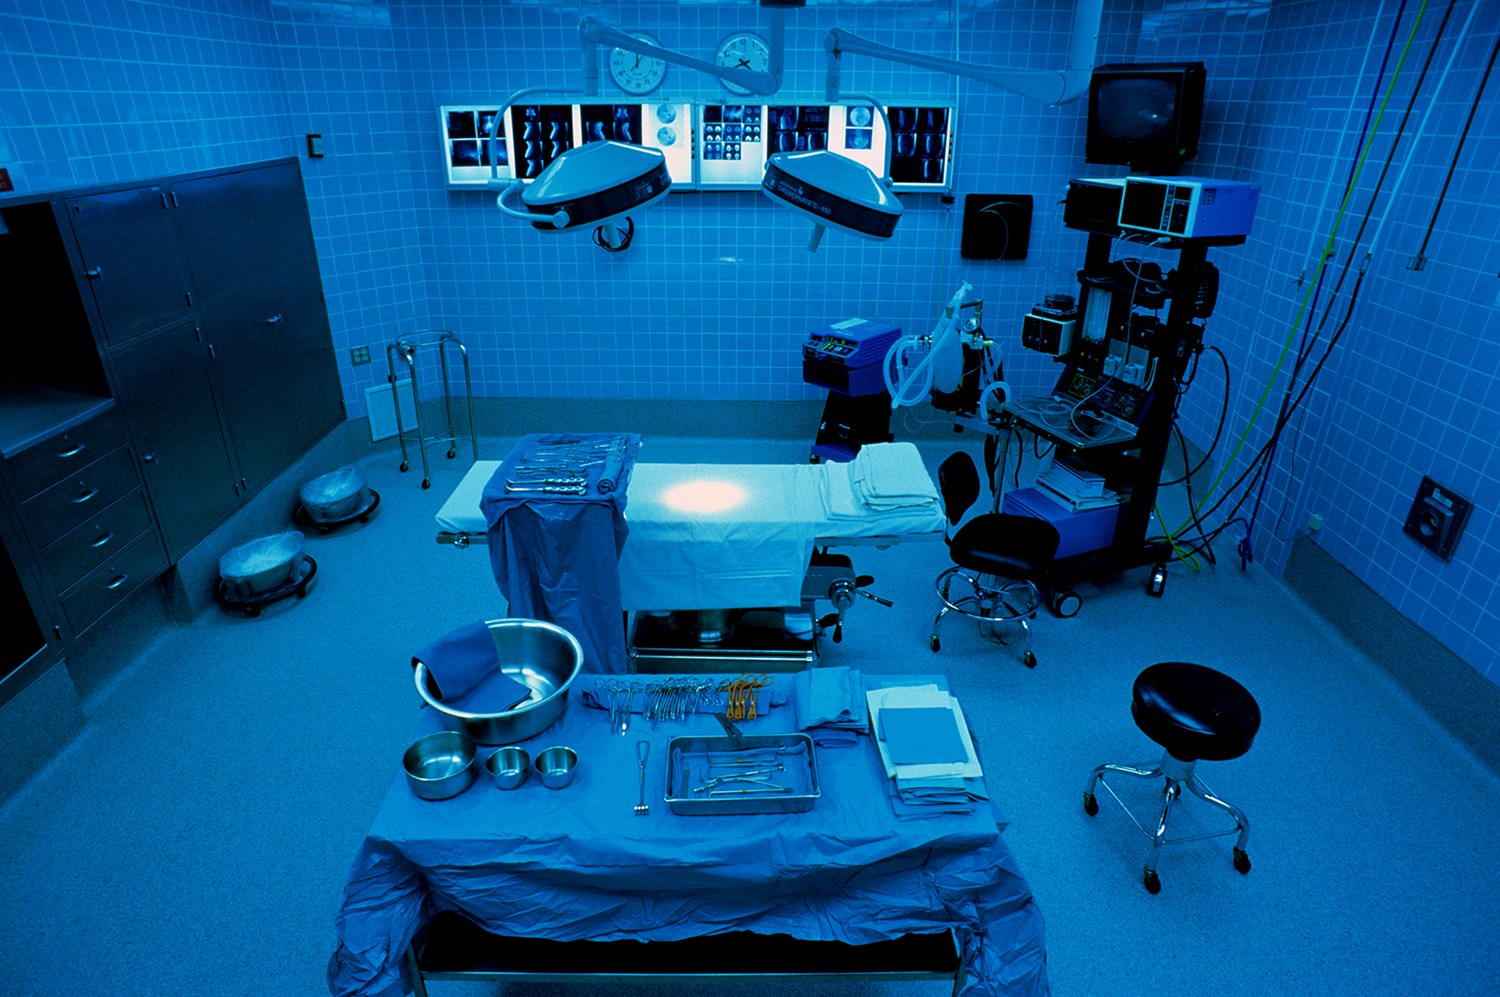
\includegraphics[height=.3\textheight]{figures/hospital-hacking.jpg}
                \caption{``It's Insanely Easy to Hack Hospital Equipment'' \cite{zetter_its_2014}}
                % zetter_its_2014: picture and article
                \label{hack_hospital}
            \end{figure}
            % \pause
            % \begin{itemize}
            %     \item Remote control of equipment
            % \end{itemize}
        \end{column}
        \pause
        \begin{column}{0.5\textwidth}
            \begin{figure}
                \centering
                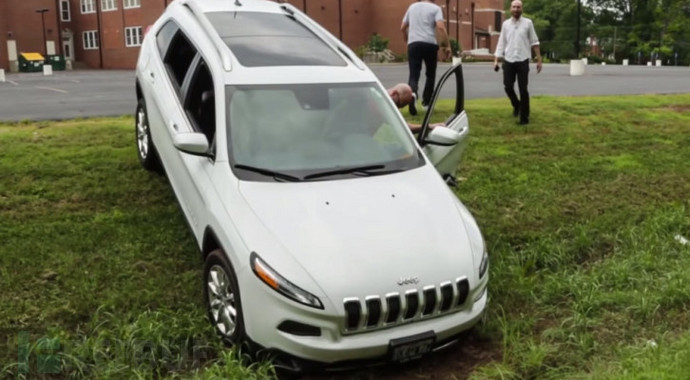
\includegraphics[height=.3\textheight]{figures/jeep_offroad.jpg}
                \caption{``Remote Exploitation of an Unaltered Passenger Vehicle'' \cite{greenberg_hackers_2015,miller_remote_2015}}
                % greenberg_hackers_2015: picture
                % miller_remote_2015: white paper
                \label{jeep_offroad}
            \end{figure}
            % \pause
            % \begin{itemize}
            %     \item Total control of drive systems
            % \end{itemize}
        \end{column}
    \end{columns}
\end{frame}

% \begin{frame}{Security critical systems - vulnerable}
%     Vulnerabilities are caused by:
%     \begin{itemize}
%         \item Increased surface of attack (more and more features, codebases explode in size)
%         \item Connected to networks $\rightarrow$ remote attacks
%     \end{itemize}

%     \note{Often a result of misconfiguration.}
% \end{frame}

\begin{frame}{Secure execution platforms}
    \begin{columns}
        \begin{column}{0.4\textwidth}
            \begin{center}
                
\includegraphics[height=2cm]{logos/seL4-logo-text-white.png}
            \end{center}
            \only<1>{
                \bigskip
                \begin{center}
                    \huge\textbf{\color{blue}{MINIX 3}}
                \end{center}
            }
        \end{column}
        \begin{column}{0.6\textwidth}
            \only<1>
            {
                \begin{center}
                    
\includegraphics[width=4cm]{logos/Integrity_Multivisor.jpg}
                \end{center}
                \bigskip
                \bigskip
                \begin{center}
                    
\includegraphics[height=1.1cm]{logos/microsoft-logo.png}\\
                    \large\textbf{Hyper-V}
                \end{center}
            }
            \only<2-4>
            {
                \visible<3->{
                    Formal proof \cite{noauthor_what_nodate}:
                    \begin{itemize}
                        \item The binary code correctly implements its \textbf{abstract specification}.
                        \item The specification guarantees \textbf{integrity} and \textbf{confidentiality}.
                    \end{itemize}
                    }

                \bigskip

                \visible<4->{
                    \begin{itemize}
                        \item \textbf{Integrity}: data cannot be \textit{changed} without permission.
                        \item \textbf{Confidentiality}: data cannot be \textit{read} without permission.
                    \end{itemize}
                }
            }
        \end{column}
    \end{columns}
\end{frame}

\begin{frame}{Secure operating systems}
    \begin{columns}
        \begin{column}{0.4\textwidth}
            \begin{center}
                
\includegraphics[height=2cm]{logos/seL4-logo-text-white.png}
            \end{center}
        \end{column}
        \begin{column}{0.6\textwidth}
            Proof assumptions \cite{noauthor_is_nodate}:
            \pause
            \begin{itemize}
                \item Use of Direct Memory Access (DMA) is excluded, or only allowed for \textbf{trusted drivers that have to be formally verified by the user}.
            \end{itemize}

            \note{Ongoing work: IOMMUs on x86 or System MMUs on ARM.}
        \end{column}
    \end{columns}
\end{frame}

\begin{frame}{What is DMA?}
    \begin{center}
        \begin{figure}
            \only<1|handout:0>{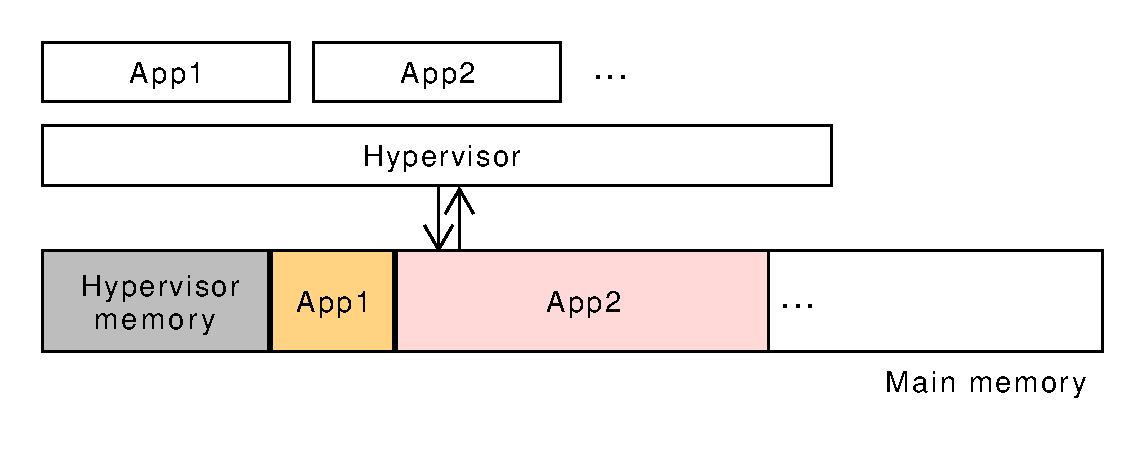
\includegraphics[width=\textwidth]{figures/dma-hyp-apps-nodma.pdf}}
            \only<2>{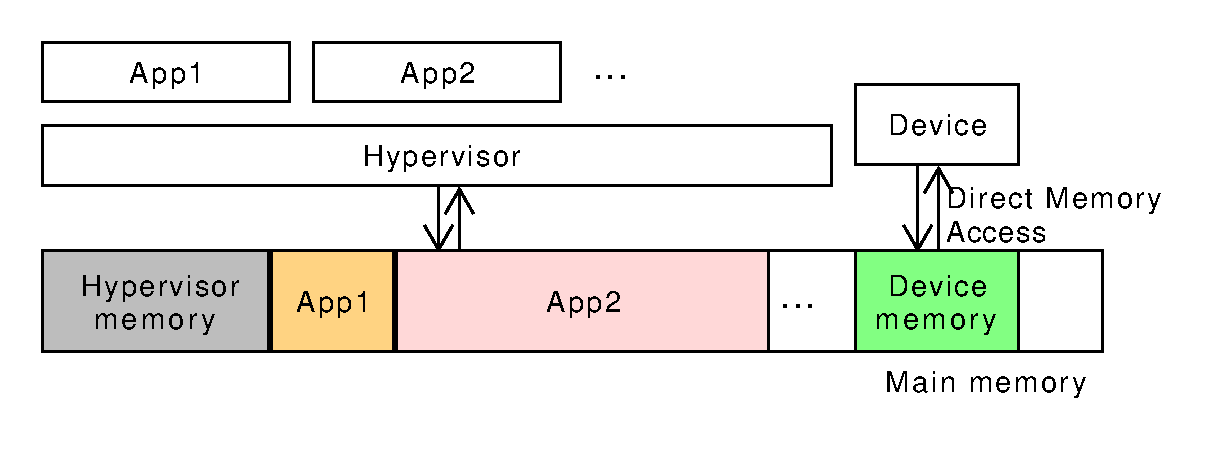
\includegraphics[width=\textwidth]{figures/dma-hyp-apps.pdf}}
            \label{dma-dangers-1}
        \end{figure}
    \end{center}
\end{frame}

%%%%%%%%%%%%%%%%%%%%%%%%%%%%%%%%%%%%%%%%%%%%%%%%%%%%%%%%%%%%%%%%%%%%%%%%%%%%%%%%

\subsection{Formal verification}

\begin{frame}{System software verification}
    \textbf{Objective}: show absence of errors in modelisation of real systems
    \bigskip
    \pause

    \begin{columns}[T]
        \begin{column}{0.5\textwidth}
            \textbf{Formal proof \phantom{long long long title}}

            machine checkable proofs using rigorous semantic
            \phantom{needs 3 lines to align}

            \bigskip
            Use small reliable kernels \\
            $\rightarrow$ produced theorems are trustworthy

            \bigskip
            \textit{Examples}: HOL4, Coq, Isabelle

            % From ITP course:
            \note{However complicated and potentially buggy your code is, if a value of type theorem is produced, it has been created through the small trusted interface. Therefore the statement really holds.}
        \end{column}
        \pause
        \begin{column}{0.5\textwidth}
                \textbf{Non proof-producing verification}

                specialized programs or procedures that check a given property

            \bigskip
            Classic bug-prone software\\
            $\rightarrow$ need tests, less trustworthy \phantom{one more line}

            \bigskip
            SMT solvers, model checkers
        \end{column}
    \end{columns}

    \note{Also: model checking}
\end{frame}

%%%%%%%%%%%%%%%%%%%%%%%%%%%%%%%%%%%%%%%%%%%%%%%%%%%%%%%%%%%%%%%%%%%%%%%%%%%%%%%%

\subsection{Network Interface Controllers (NIC)}

\begin{frame}{Network Interface Controller (NIC)}
    \begin{figure}
        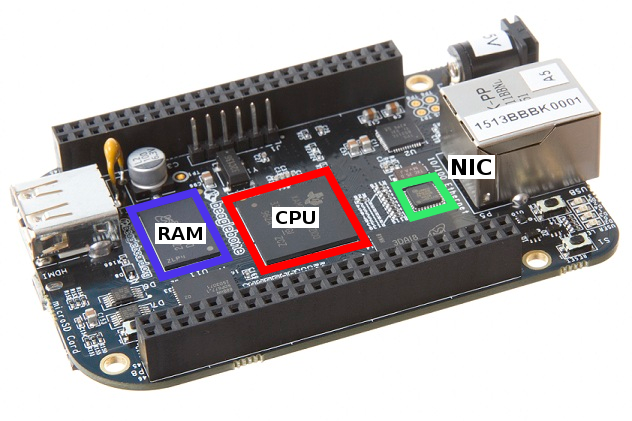
\includegraphics[]{figures/BBB_cpu_ram_nic.png}
        \caption{BeagleBone Black.}
        \label{bbb_nic}
    \end{figure}
\end{frame}

\begin{frame}{NIC: How it works}
    \begin{figure}
        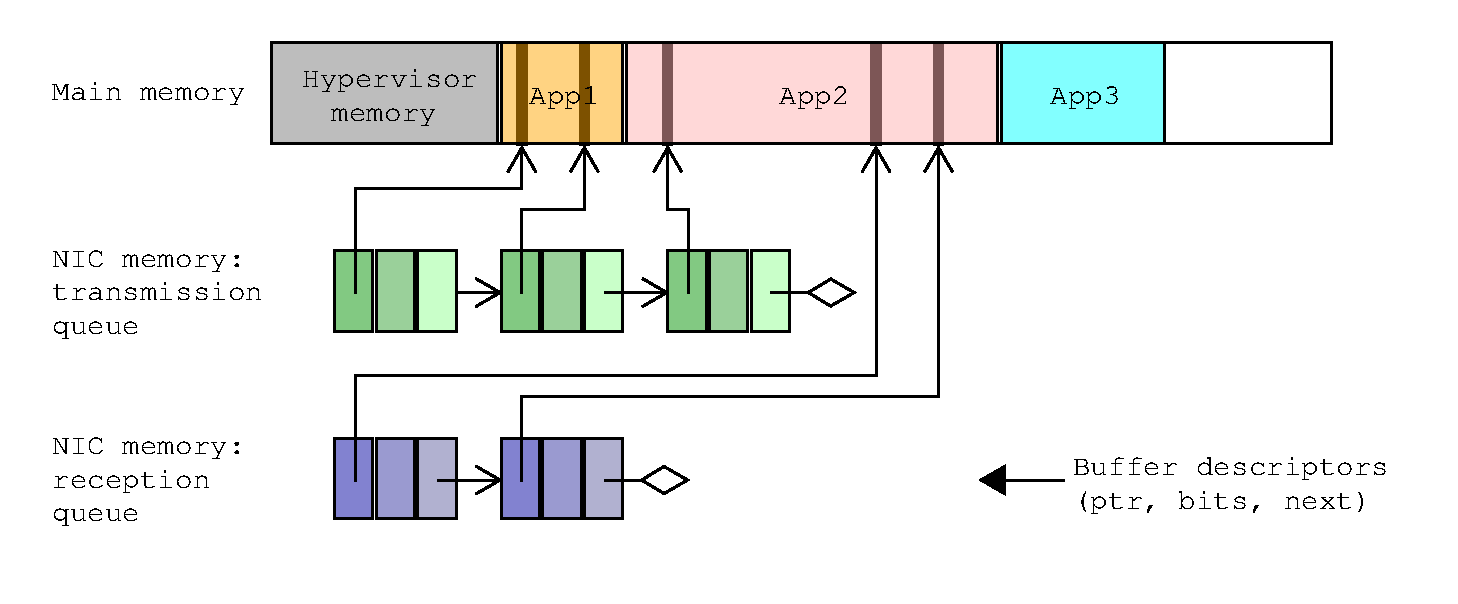
\includegraphics[width=\textwidth]{figures/nic-bd.pdf}
        \label{nic_bd}
    \end{figure}
\end{frame}

\begin{frame}{NIC: How it works}
    \begin{figure}
        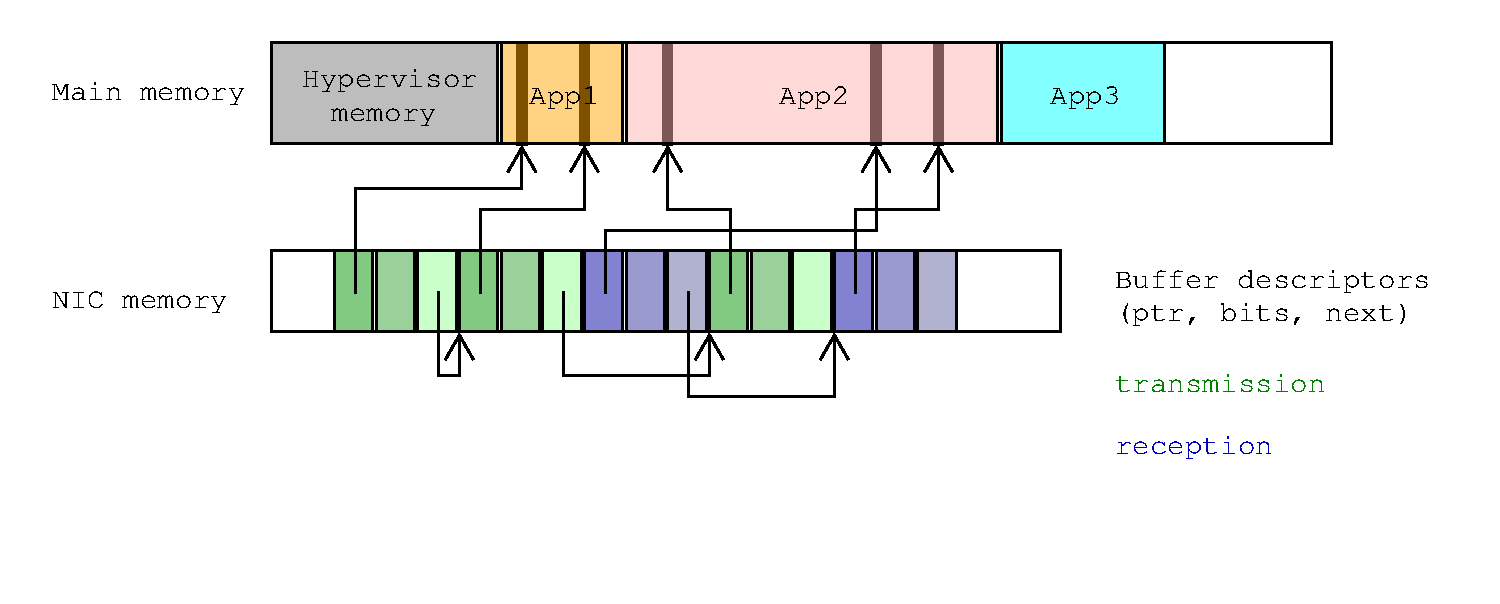
\includegraphics[width=\textwidth]{figures/nic-bd-in_mem.pdf}
        \label{nic_bd_inmem}
    \end{figure}
\end{frame}

\begin{frame}{NIC: How it can fail}
    \begin{figure}
        \includegraphics<1>[width=\textwidth]{figures/nic-bd-in_mem-overlap1.pdf}
        \includegraphics<2>[width=\textwidth]{figures/nic-bd-in_mem-overlap2.pdf}
        \includegraphics<3>[width=\textwidth]{figures/nic-bd-in_mem-overlap3.pdf}
        \label{nic_bd_inmem_overlap}
    \end{figure}
    \note{Figure 32 in Jonas' MT}
    \note{also: not circular}
\end{frame}

\begin{frame}{NIC: How it has been modeled \cite{haglund_formal_2016}}
    \begin{columns}
        \begin{column}{0.5\textwidth}
            \begin{center}
                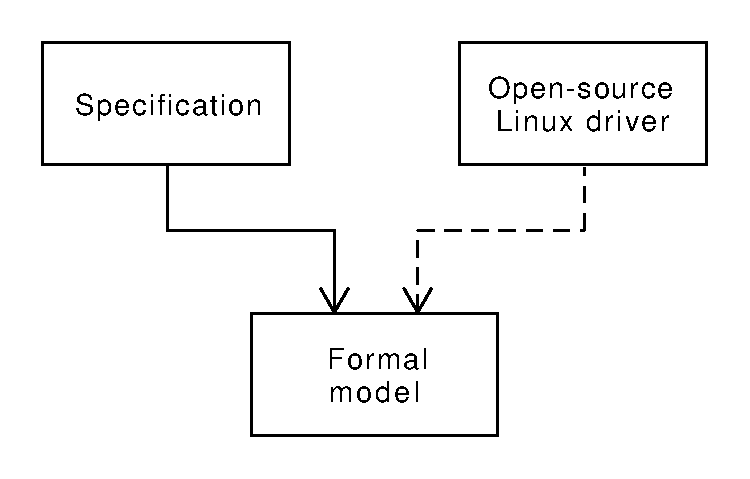
\includegraphics[width=\columnwidth]{figures/nic_how_modeled.pdf}
            \end{center}
        \end{column}
        \pause
        \begin{column}{0.5\textwidth}
            Transition system:

            \begin{center}
                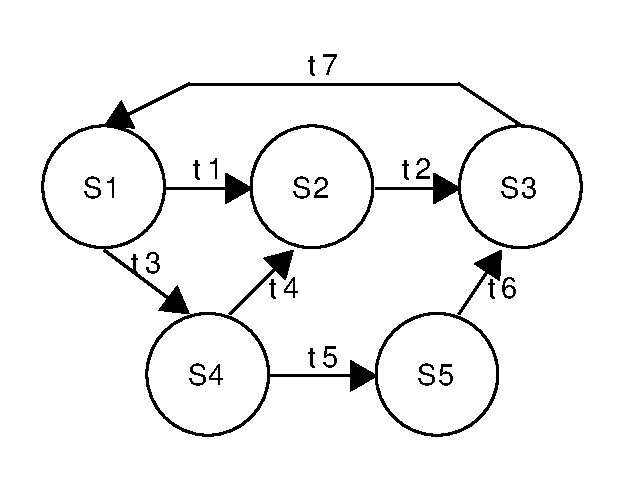
\includegraphics[width=.8\columnwidth]{figures/transition_sys.pdf}
            \end{center}

            \note{The model describes these operations to the extent that they are used by the device driver of the NIC in Linux 3.10. The NIC is modeled as a transition system where each transition corresponds to one operation that accesses one field or byte of a NIC register or the memory.}
        \end{column}
    \end{columns}
    % \pause
    % \begin{center}
    %     Unspecified behavior $\rightarrow$ ``dead'' state
    % \end{center}
\end{frame}

\begin{frame}{Hoare Triple}
    \begin{center}
        \begin{equation*}
            \forall S.~P(S)~\land~S'=program(S)~\implies~Q(S')
        \end{equation*}
    \end{center}
    \begin{columns}
        \begin{column}{.5\textwidth}
            \begin{center}
                \begin{tikzpicture}
                    \matrix [matrix of nodes,ampersand replacement=\&, column sep=20mm]{
                        \node (a) [draw,label={P},shape=circle] {$S$}; \&
                        \node (b) [draw,label={Q},shape=circle] {$S'$}; \\
                    };
                    \draw[->,thick] (a) -- node[auto] {$program$} (b);
                \end{tikzpicture}
            \end{center}
        \end{column}
        \begin{column}{.5\textwidth}
            \begin{center}
                \begin{equation*}
                    \{P\} ~ program ~ \{Q\}
                \end{equation*}
                \bigskip
            \end{center}
        \end{column}
    \end{columns}
\end{frame}

\begin{frame}{Weakest precondition}
    \begin{center}
        \textit{Weakest} precondition $WP$ such that:
        \begin{equation*}
            \htriple{WP}{program}{Q}
        \end{equation*}
        
        \begin{equation*}
            \Big(\forall S.~P(S) \implies WP(S)\Big) \implies \htriple{P}{program}{Q}
        \end{equation*}

        \bigskip
        \pause

        \begin{equation*}
            \WP = f(program,~Q)
        \end{equation*}
    \end{center}
\end{frame}

\begin{frame}<-7>{NIC: What the verification looks like \cite{haglund_formal_2016}}
    \only<8->{\setbeamercovered{transparent}}

    \uncover<2->{
        Low-level lemmas:
        \begin{itemize}
            \item<3-8> \htriple{\neg dead \land well\_configured}{transition}{\neg dead}
            \item<4-8> \htriple{\neg overlapping \land \neg cyclic}{transition}{\neg overlapping}
            \item<5-8> \htriple{\neg overlapping \land \neg cyclic}{transition}{\neg cyclic}
        \end{itemize}
    }

    \bigskip

    \uncover<6-7>{
        Intermediate lemmas:
        \begin{itemize}
            \item \textit{\small Invariant}: $rx\_invariant\_well\_defined$
            \item \textit{\small Invariant}: $tx\_invariant\_well\_defined$
        \end{itemize}
    }

    \bigskip

    \uncover<7-7>{
        Security theorems:
        \begin{itemize}
            \item $\forall~tx\_bd.~readable(tx\_bd)$ ~~~~~~~ \textit{\tiny BD = Buffer Descriptor}
            \item $\forall~rx\_bd.~writable(rx\_bd)$
        \end{itemize}
    }

    \note{Cannot express forall with BIR, and ``QF_AUFBV''}
\end{frame}

\begin{frame}{Research question}
    \begin{center}
        \textbf{Can we apply traditional software verification techniques and tools to show security properties of hardware devices?}
    \end{center}
\end{frame}

\begin{frame}{HolBA: HOL4 Binary Analysis platform}
    \begin{itemize}%[<+->]
        \item Verification platform at binary level
        \item Centered around its Intermediate Language, BIR
        \item Features proof-producing tools
              \begin{itemize}
                  \item Weakest precondition generation
              \end{itemize}
    \end{itemize}
\end{frame}

%%%%%%%%%%%%%%%%%%%%%%%%%%%%%%%%%%%%%%%%%%%%%%%%%%%%%%%%%%%%%%%%%%%%%%%%%%%%%%%%
%%%%%%%%%%%%%%%%%%%%%%%%%%%%%%%%%%%%%%%%%%%%%%%%%%%%%%%%%%%%%%%%%%%%%%%%%%%%%%%%
%%%%%%%%%%%%%%%%%%%%%%%%%%%%%%%%%%%%%%%%%%%%%%%%%%%%%%%%%%%%%%%%%%%%%%%%%%%%%%%%

\section{Automatic contract-based verification}

\subsection{Pipeline}

\begin{frame}{Contract-based verification pipeline}
    \begin{columns}
        \begin{column}[T]{.5\textwidth}
            \begin{enumerate}
                \item[0.]<1-> Translate the model in BIR
                \item[1.]<2-> Formulate a Hoare Triple
                \item[2.]<3-> Translate P and Q to BIR
                \item[3.]<4-> Generate the WP
                \item[4.]<7-> Translate the goal into a SMT-compatible expression
            \end{enumerate}

            \bigskip
            \begin{center}
                \only<1>{$transition_{BIR}$}
                \only<2>{\htriple{P}{transition_{BIR}}{Q}}
                \only<3>{\htriple{P_{BIR}}{transition_{BIR}}{Q_{BIR}}}
                \only<4>{$P_{BIR}(S) \implies \WP_{BIR}(S)$}
                \only<5>{
                    \textbf{S}atisfiability \textbf{M}odulo \textbf{T}heories
                    \begin{itemize}
                        \item external tools \phantom{left left}
                        \item SMT-LIB 2.0
                    \end{itemize}
                }
                \only<6>{
                    $\neg\Big(P_{BIR}(S) \implies \WP_{BIR}(S)\Big)$
                    \bigskip

                    ``unsat''?
                }
                \only<7>{
                    $\neg\Big(P(S) \implies \WP(S)\Big)_{SMT}$
                    \bigskip

                    ``unsat''?
                }
            \end{center}
        \end{column}
        \begin{column}[T]{.6\textwidth}
            \vspace{-1cm}
            \begin{center}
                \includegraphics<1>[height=.8\textheight]{figures/pipeline-0.pdf}
                \includegraphics<2>[height=.8\textheight]{figures/pipeline-1.pdf}
                \includegraphics<3>[height=.8\textheight]{figures/pipeline-2.pdf}
                \includegraphics<4>[height=.8\textheight]{figures/pipeline-3.pdf}
                \includegraphics<5>[height=.8\textheight]{figures/pipeline-3-1.pdf}
                \includegraphics<6>[height=.8\textheight]{figures/pipeline-4.pdf}
                \includegraphics<7>[height=.8\textheight]{figures/pipeline-all.pdf}
            \end{center}
        \end{column}
    \end{columns}
\end{frame}

\subsection{How trustful is it?}

\begin{frame}{How trustful is it?}
    \begin{columns}
        \begin{column}{.5\textwidth}
            \begin{itemize}
                \setlength\itemsep{1em}
                \item<2-> SMT solvers don't produce proofs
                \item<3-> bir2bool isn't proof-producing
                % \item<4-> The BIR model may be wrong
            \end{itemize}
        \end{column}
        \begin{column}{.6\textwidth}
            \begin{center}
                \includegraphics<1>[height=.8\textheight]{figures/pipeline-all.pdf}
                \includegraphics<2>[height=.8\textheight]{figures/pipeline-all-trustful-1.pdf}
                \includegraphics<3>[height=.8\textheight]{figures/pipeline-all-trustful-2.pdf}
                % \includegraphics<4>[height=.8\textheight]{figures/pipeline-all-trustful-3.pdf}
            \end{center}
        \end{column}
    \end{columns}
\end{frame}

\subsection{How powerful is it?}

\begin{frame}{How powerful is it?}
    \begin{block}<2->{Not proof-producing}
        Easier non-proof producing platforms exist
    \end{block}
    \begin{block}<3->{Limited by SMT solvers' logics}
        \begin{itemize}
            \item<4-> \htriple{\neg overlapping \land \neg cyclic}{transition}{\neg overlapping}
            \item<5-> SMT logic: \textbf{QF}\_AUFBV $\rightarrow$ \textbf{Q}uantifier-\textbf{F}ree
        \end{itemize}
    \end{block}
    \begin{block}<6->{Cannot compose theorems}
        \begin{itemize}
            \item<7-> Work in progress in HolBA
            % \item<8-> Need theorems to compose trustfully
        \end{itemize}
    \end{block}
\end{frame}

\section{Proof-producing verification}

\begin{frame}{Goal}
    \begin{itemize}
        \item[$\rightarrow$]<2-> Some theorems cannot be proved with previous pipeline
        \item[$\rightarrow$]<3-> We would like to prove them anyway
        \item[$\rightarrow$]<4-> We want to use them with the current proof
    \end{itemize}

    % \tikzset{every label/.style={opacity=0.5}}
    \begin{center}
        \begin{tikzpicture}
            \matrix [matrix of nodes,ampersand replacement=\&, column sep=25mm,row sep=10mm]{
                \node (a) [draw,label={120:$P$},shape=circle,visible on=<5->] {$S$}; \&
                \node (b) [draw,label={40:$Q$},shape=circle,visible on=<5->] {$S'$}; \\
                \node (c) [draw,label={210:$P_{BIR}$},shape=circle,visible on=<6->] {$B$}; \&
                \node (d) [draw,label={-50:$Q_{BIR}$},shape=circle,visible on=<6->] {$B'$}; \\
            };
            \draw[->,thick,dashed,visible on=<5->] (a) -- node[auto] {$formal~model$} (b);
            \draw[->,thick,visible on=<6->] (c) -- node[auto] {$BIR~program$} (d);
            \draw[->,thick,visible on=<7->] (a) -- node[auto] {} (c);
            \draw[->,thick,visible on=<7->] (d) -- node[auto] {} (b);
        \end{tikzpicture}
    \end{center}
\end{frame}

\begin{frame}{Goal}
    \begin{columns}
        \begin{column}{.6\columnwidth}
            \begin{center}
                \uncov<1,5>{
                    \htriple{P}{BIR\_prog}{Q}

                    \medskip
                    $\equiv$
                    \medskip

                    $\forall S~S'.~\mathbf{exec}~S~BIR\_prog~S'$\\
                    $\implies \mathbf{P}~S \implies \mathbf{Q}~S'$
                }

                \bigskip
                \bigskip

                \uncover<2->{
                    $\uncov<2,5>{\forall S~S'.~\mathbf{exec}~S~BIR\_prog~S'\eqdef}$\\
                    $~~\uncov<5>{\forall B~B'.} (\uncov<3,5>{B' = \mathbf{BIR\_exec}~BIR\_prog~B}$\\
                    $~~~\uncov<4,5>{\land~\mathbf{R}~S~B}) \uncov<4,5>{\implies \mathbf{R}~S'~B'}$
                }
            \end{center}
        \end{column}
        \begin{column}{.4\columnwidth}
            \begin{center}
                \begin{tikzpicture}[every text node part/.style={align=center}]
                    \matrix [matrix of nodes,ampersand replacement=\&, column sep=25mm,row sep=10mm]{
                        \node (a) [draw,label={[von={<1,5>}]90:$P$},shape=circle,von={<1,2,4,5>}] {$S$}; \&
                        \node (b) [draw,label={[von={<1,5>}]90:$Q$},shape=circle,von={<1,2,4,5>}] {$S'$}; \\
                        \node (c) [draw,label={[opacity=.2]-90:$P_{BIR}$},shape=circle,von={<3,4,5>}] {$B$}; \&
                        \node (d) [draw,label={[opacity=.2]-90:$Q_{BIR}$},shape=circle,von={<3,4,5>}] {$B'$}; \\
                    };
                    \draw[->,thick,dashed,von={<2,5>}] (a) -- node[auto] {$formal~model$ \\ \small(a)} (b);
                    \draw[->,thick,von={<1,2,3,5>}] (c) -- node[auto,below] {$BIR~program$ \\ \small(c)} (d);
                    \draw[->,thick,von={<4,5>}] (a) -- node[auto] {\small (b)} (c);
                    \draw[->,thick,von={<4,5>}] (d) -- node[auto] {\small (d)} (b);
                \end{tikzpicture}
            \end{center}
        \end{column}
    \end{columns}
\end{frame}

\begin{frame}<-11>{Proof overview}
    \begin{columns}
        \begin{column}{.6\columnwidth}
            \only<9>{\raggedright
                Notation: $\mathbf{P_{BIR}}~B~\eqdef~\mathbf{BIR\_eval}~P_{BIR}~B$
                \bigskip

                % Where:
                % \begin{itemize}
                %     \item[-] $B$ is a BIR state % this is true enough for this presentation (it's an env)
                %     \item[-] $P_{BIR}$ is a BIR expression
                % \end{itemize}

                \note{
                    Explains why $Q_{BIR}~B~B'$ is impossible: \mathbf{BIR\_eval} has a fixed arity,
                    where $P$ and $Q$ have been arbitrarily defined
                }
            }
            \only<2-8,10->{
                \begin{itemize}
                    \item<2->[\alt<-10>{(a)}{1.}] \cov<3-9,11>{
                        $\forall S~S'.~\mathbf{exec}~S~BIR\_prog~S'\eqdef$\\
                        $~~\forall B~B'. (B' = \mathbf{BIR\_exec}~BIR\_prog~B$\\
                        $~~~\land~\mathbf{R}~S~B) \implies \mathbf{R}~S'~B'$
                    }
                    \item<3->[\alt<-10>{--~}{2.}] \cov<4-9,11>{Relation between $S$ and $B$: $\mathbf{R}~S~B$}
                    \item<4->[\alt<-10>{(b)}{3.}] \cov<5-9,11>{Injectivity: $\forall S.~\exists B.~\mathbf{R}~S~B$}
                    \item<5->[\alt<-10>{(b)}{4.}] \cov<6-9,11>{$\forall B.~(\exists S.~\mathbf{R}~S~B \land \mathbf{P}~S) \implies \mathbf{P_{BIR}}~B$}
                    \item<6->[\alt<-10>{(c)}{5.}] \cov<8-9,11>{\alt<-6>{
                        % 6
                        $\forall B~B'.~(\mathbf{P_{BIR}}~B \land B'=\mathbf{BIR\_exec}~BIR\_prog~B) \implies \mathbf{Q_{BIR}}~B'$
                    }{
                        % 7
                        \htriple{P_{BIR}}{BIR~program}{Q_{BIR}}
                    }}
                    \item<8->[\alt<-10>{(d)}{6.}] \cov<11>{
                        $\forall B'.~\mathbf{Q_{BIR}}~B' \implies$\\
                        $(\forall S~S'~B.~\mathbf{P_{BIR}}~B \land \mathbf{R}~S~B~\land~\mathbf{R}~S'~B'$\\
                        $\implies \mathbf{Q}~S~S')$
                    }
                \end{itemize}
            }
        \end{column}
        \begin{column}{.4\columnwidth}
            \begin{center}
                \begin{tikzpicture}[every text node part/.style={align=center}]
                    \matrix [matrix of nodes,ampersand replacement=\&, column sep=25mm,row sep=10mm]{
                        \node (a) [draw,label={[von={<1,5,10>}]90:$P$},shape=circle,von={<1,2,3,4,5,10>}] {$S$}; \&
                        \node (b) [draw,label={[von={<1,8-9,10>}]90:$Q$},shape=circle,von={<1,2,3,8-9,10>}] {$S'$}; \\
                        \node (c) [draw,label={[von={<1,5,6-7,8-9,10>}]-90:$P_{BIR}$},shape=circle,von={<1,2,3,4,5,6-7,8-9,10>}] {$B$}; \&
                        \node (d) [draw,label={[von={<1,6-7,8-9,10>}]-90:$Q_{BIR}$},shape=circle,von={<1,2,3,6-7,8-9,10>}] {$B'$}; \\
                    };
                    \draw[->,thick,dashed,von={<1,2,10>}] (a) -- node[auto] {$formal~model$ \\ \small(a)} (b);
                    \draw[->,thick,von={<1,6-7,10>}] (c) -- node[auto,below] {$BIR~program$ \\ \small(c)} (d);
                    \draw[->,thick,von={<1,3,4,5,10>}] (a) -- node[auto] {\small (b)} (c);
                    \draw[->,thick,von={<1,3,8-9,10>}] (d) -- node[auto] {\small (d)} (b);
                \end{tikzpicture}
            \end{center}
        \end{column}
    \end{columns}
\end{frame}

\begin{frame}{Proof overview - automate?}
    \begin{table}[]
        \begin{tabular}{|l|c|c|}
        \hline
        Theorem & Length of proof (LoC) & Ease to automate \\
        \hline
        \hline
        1. def $S \rightarrow S'$ \textit{\small (a)} & -- & \textit{Hard?} \textit{(lifter)} \\ \hline
        2. def relation \textit{\small (R)} & -- & Easy \\ \hline
        3. Injectivity & 10 & Very easy \\ \hline
        4. $P \rightarrow P_{BIR}$ \textit{\small (b)} & 4 & Very easy \\ \hline
        5. Hoare Triple \textit{\small (c)} & 151 & \textit{Medium?} *$^{2}$ \\ \hline
        6. $Q_{BIR} \rightarrow S$ \textit{\small (d)} & 48 & Should be easy *$^{1}$ \\ \hline
        \end{tabular}
    \end{table}

    \visible<2->{*$^{1}$ Need 2 simple tactics}

    \visible<3->{*$^{2}$ Need smart tactics (multi-pass, goal aware)}
\end{frame}

%%%%%%%%%%%%%%%%%%%%%%%%%%%%%%%%%%%%%%%%%%%%%%%%%%%%%%%%%%%%%%%%%%%%%%%%%%%%%%%%
%%%%%%%%%%%%%%%%%%%%%%%%%%%%%%%%%%%%%%%%%%%%%%%%%%%%%%%%%%%%%%%%%%%%%%%%%%%%%%%%
%%%%%%%%%%%%%%%%%%%%%%%%%%%%%%%%%%%%%%%%%%%%%%%%%%%%%%%%%%%%%%%%%%%%%%%%%%%%%%%%

\section{Conclusion}

\begin{frame}{Conclusion}
    \begin{itemize}
        \item Automation is feasible
        \item Can reduce proof lengths and complexity
        \item Trustworthy if proof-producing
    \end{itemize}
\end{frame}

\begin{frame}
    \begin{center}
        \huge
        Questions
    \end{center}
\end{frame}

%%%%%%%%%%%%%%%%%%%%%%%%%%%%%%%%%%%%%%%%%%%%%%%%%%%%%%%%%%%%%%%%%%%%%%%%%%%%%%%%
%%%%%%%%%%%%%%%%%%%%%%%%%%%%%%%%%%%%%%%%%%%%%%%%%%%%%%%%%%%%%%%%%%%%%%%%%%%%%%%%
%%%%%%%%%%%%%%%%%%%%%%%%%%%%%%%%%%%%%%%%%%%%%%%%%%%%%%%%%%%%%%%%%%%%%%%%%%%%%%%%

\appendix

\begin{frame}[allowframebreaks]{References}
    \nocite{*}
    \setbeamertemplate{bibliography item}{\insertbiblabel}
    \bibliographystyle{plain}
    % \bibliographystyle{IEEEtran}
    \bibliography{ref-slides}
\end{frame}

\begin{frame}{HolBA overview}
    \begin{figure}
        \centering
        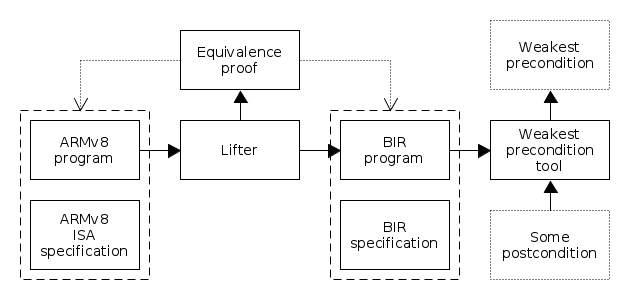
\includegraphics[height=4cm]{../figures/holba-overview.png}
        \caption{Overview of the HolBA framework (lifter and WP tool)}
    \end{figure}
\end{frame}

\begin{frame}{Fringe}
    \begin{figure}
        \centering
        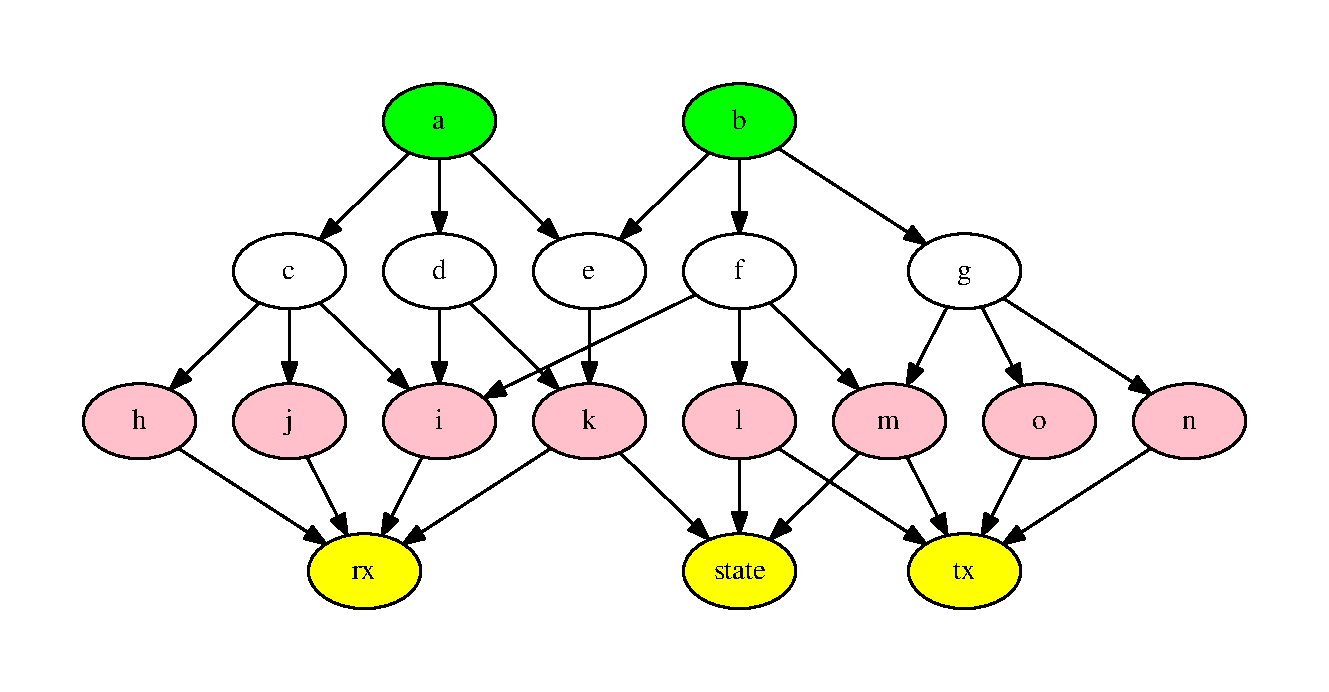
\includegraphics[height=5cm]{../figures/fringe.pdf}
        \caption{Fringe of an ideally-shaped proof}
    \end{figure}
\end{frame}

\begin{frame}[fragile]{Pipeline public interface}
    \begin{lstlisting}[
        language=Caml,
        frame=tb,
        backgroundcolor=\color{codebackcolour},
        commentstyle=\color{codegreen},
        keywordstyle=\color{magenta},
        stringstyle=\color{codepurple}
    ]
val thm = prove_contract "cjmp"
  cjmp_prog_def
  (* Precondition *) (blabel_str "entry", btrue)
  (* Postcondition *) (
    [blabel_str "end"],
    beq ((bden o bvarimm32) "y", bconst32 100)
  )
    \end{lstlisting}
\end{frame}

\begin{frame}[fragile]{BSL: BIR Simple Language}
    \begin{lstlisting}[
        language=Caml,
        basicstyle=\footnotesize\ttfamily,
        frame=tb,
        backgroundcolor=\color{codebackcolour},
        commentstyle=\color{codegreen},
        keywordstyle=\color{magenta},
        stringstyle=\color{codepurple}
    ]
bite (
  borl [
    ble ((bden o bvarimm64) "x", bconst64 100),
    bnot (ble (bplus ((bden o bvarimm64) "y", bconst64 1),
               bconst64 10)),
    ble (bplus ((bden o bvarimm64) "x",
                (bden o bvarimm64) "y"),
         bconst64 20)
  ],
  bmult ((bden o bvarimm64) "x", bconst64 2),
  bplus (bmult ((bden o bvarimm64) "x", bconst64 3),
         bconst64 1)
)
    \end{lstlisting}
\end{frame}

\begin{frame}{BIR pretty-printer - disabled}
    \begin{figure}
        \centering
        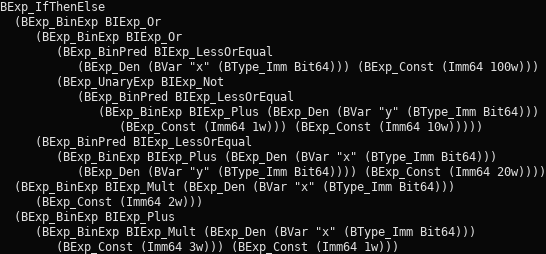
\includegraphics[height=5cm]{../figures/pp_ex_default_printing.png}
    \end{figure}
\end{frame}

\begin{frame}{BIR pretty-printer - enabled}
    \begin{figure}
        \centering
        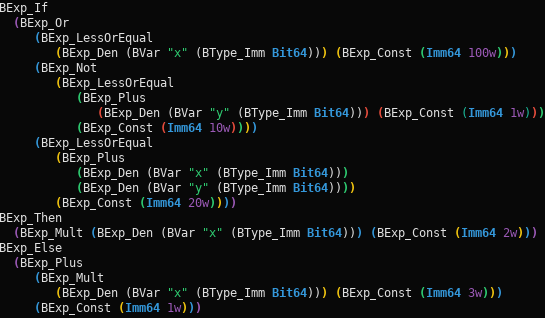
\includegraphics[height=5cm]{../figures/pp_ex_pretty_printing.png}
    \end{figure}
\end{frame}

\begin{frame}{Exception pretty-printer and LogLib}
    \begin{figure}
        \centering
        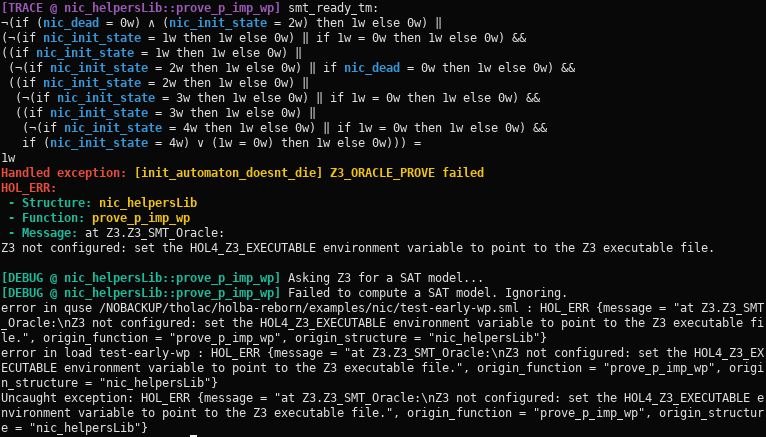
\includegraphics[height=5cm]{../figures/loglib-ppexn-ppterm.png}
    \end{figure}
\end{frame}

\begin{frame}{Continuous Integration (CI) - tests}
    \begin{figure}
        \centering
        
\includegraphics[height=2cm]{figures/ci_tests.png}
    \end{figure}
\end{frame}

\begin{frame}{Continuous Integration (CI) - static analysis}
    \begin{figure}
        \centering
        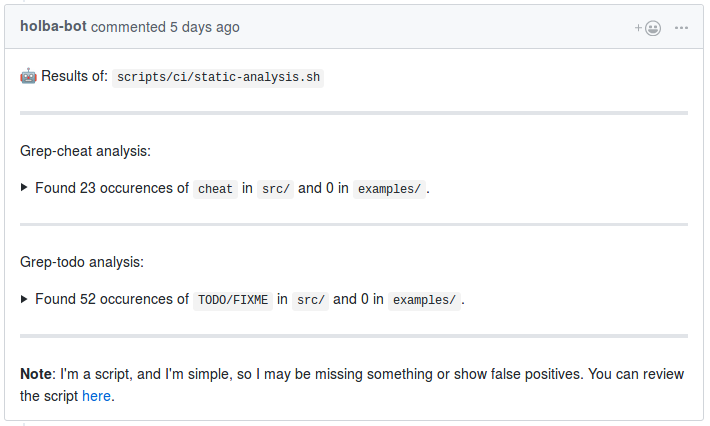
\includegraphics[height=5cm]{figures/ci_static_analysis.png}
    \end{figure}
\end{frame}

% \begin{frame}{Other work}
%     \begin{itemize}
%         \item \textbf{TODO}: Pictures of BSL
%         \item \textbf{TODO}: Pictures of interface
%         \item \textbf{TODO}: Pictures of CI
%         \item \textbf{TODO}: Some code
%     \end{itemize}
% \end{frame}

\end{document}